A \$GAS token (\cite{noauthor_gastokenio_nodate}) is an existing solution to edge Gas price volatility, using the following concept: buy/mint gas when its price is low and redeem/sell it when the price is high. Such a solution is possible thanks to the ethereum Gas refund mechanism. It is well known that when one wants to write in the blockchain, one has to pay gas. But it also works the other way around: when one free some space one receives a gas refund as a reward. The refund is not as high as the initial number of gas but if the price of the gas is volatile enough this strategy is still profitable. In theory, writing (SSTORE instruction)  in a block costs 20000 gas and then erasing the storage (by overwriting it with zeros) costs 5000 gas but refunds 10000 gas. Thus. the return of this strategy is :
$$return=-20000\cdot gas_{low}+(15000-5000)\cdot gas_{high}$$
where 
$gas_{low}$ and $gas_{high}$ are respectively: the gas price when it is low and the gas price when it is high. 

In practice,it is possible to mint \$GAS tokens by banking and deploying gas using your own smart contract or to buy such tokens on exchange plateforms. These token are : CHI, GST1 and GST2 for examples. However, this strategy has some downside.
First of all, it is accesible to everyone. A simple blockchain user might not know how to set up and use a smart contract to write and free some space. 
Second, buying a \$GAS token on an exchange does not edge the gas price properly since the price of the token is not only driven by gas price but also by offer/demand pression. 
%Here is an exmaple of the CHI \$GAS token price and the gas price itself. We clearly see that the 2 curves are not perfectly correlated :
%########
Moreover, by checking transactions on ehterscan we see that some \$GAS tokens are illiquid, which is not convinient for simple users:\\
\href{https://etherscan.io/address/0x0000000000004946c0e9f43f4dee607b0ef1fa1c}{GST2 :}\\
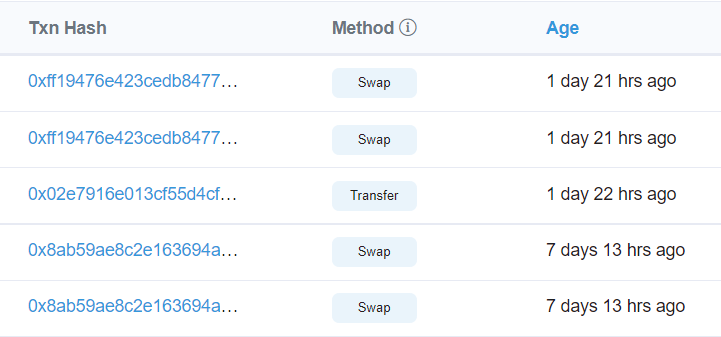
\includegraphics[width=0.45\textwidth]{figures/GST2 illiquidity.png}\\
\href{https://etherscan.io/token/0x88d60255f917e3eb94eae199d827dad837fac4cb}{GST1 : }\\
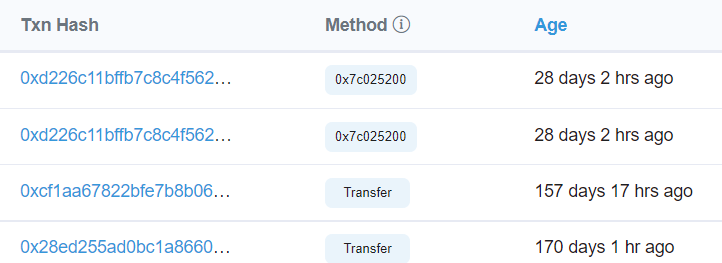
\includegraphics[width=0.45\textwidth]{figures/GST1 illiquidity.png}\\
\href{https://etherscan.io/token/0x0000000000004946c0e9f43f4dee607b0ef1fa1c}{CHI token (most liquid):}\\
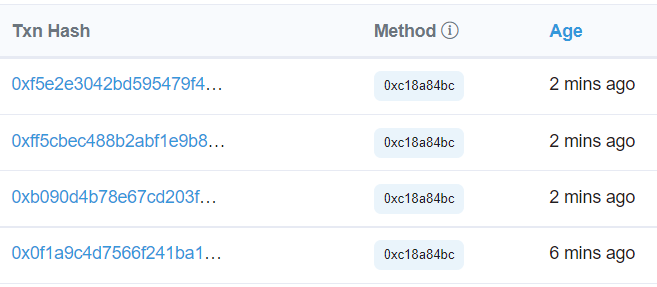
\includegraphics[width=0.45\textwidth]{figures/CHI illiquidity.png}


